% Fragment prepared for insertion into the Stokes solver section of
% /Users/tgol0006/uw_folder/UW3_benchmarks/Combined_document.tex.
% It summarises only volume L2 velocity and pressure errors from the
% annulus and spherical-shell benchmark articles.

\subsubsection{Annulus and spherical-shell Stokes benchmarks}

The Cartesian SolCx tests described above provide a controlled verification
case for Stokes flow on simple domains. We also tested the Stokes solver in
annulus and spherical-shell geometries, where the same finite-element
formulation must handle curved boundaries, radial body forces, pressure gauge
freedom, and velocity boundary conditions on non-planar surfaces. These tests
are closer to the geometries used in mantle-convection models and therefore
provide an important complement to the Cartesian benchmarks. The calculations
use the Underworld3 finite-element framework \citep{moresi_underworld3_2025}.

Only volume \(L_2\)-norm errors in velocity and pressure are summarised here.
Boundary pressure and stress diagnostics are useful in the standalone benchmark
articles, but they are not included in this combined Stokes-solver summary. For
a numerical field \(q_h\) and analytical reference solution \(q^*\), the
relative volume error is
\begin{equation}
E_{L_2}^{\mathrm{rel}}(q)
=
\left(
\frac{\int_{\Omega} |q_h-q^*|^2\,\mathrm{d}\Omega}
     {\int_{\Omega} |q^*|^2\,\mathrm{d}\Omega}
\right)^{1/2}.
\end{equation}
This definition is applied to both the velocity field and pressure field.
The pressure is compared after applying a common mean-pressure gauge, because
the incompressible Stokes equations determine pressure only up to an additive
constant unless an explicit pressure reference is imposed.

\textbf{Benchmark setup}
The annulus tests use analytical solutions in polar geometry. The
Thieulot--Puckett annulus benchmark is a smooth manufactured Stokes solution
with radial gravity and tangential velocity boundary conditions. It is useful
for checking the optimal volume convergence expected from mixed finite
elements \citep{thieulot2018,girault1986femns,boffi2013}. The Kramer annulus
benchmark separates smooth volumetric forcing from delta-function forcing on an
internal circular interface, and includes both free-slip and zero-slip velocity
boundary conditions \citep{kramer2021}.

The spherical-shell tests use analytical solutions in three-dimensional shell
geometry. The Thieulot spherical benchmark tests smooth spherical-shell Stokes
flow with both constant and radially varying viscosity \citep{thieulot2017}.
The Kramer spherical benchmark again separates smooth volumetric forcing from
delta-function forcing on an internal spherical interface \citep{kramer2021}.
This distinction is important because the smooth cases test the polynomial
approximation order of the finite element spaces, whereas the delta-function
cases intentionally reduce solution regularity.

\begin{figure}[htb]
\centering

\includegraphics[width=0.95\linewidth,height=0.78\textheight,keepaspectratio]{../annulus/thieulot/figure_5_thieulot_annulus_convergence.pdf}
\caption{Velocity and pressure convergence for the Thieulot--Puckett annulus
benchmark.}
\label{fig:combined_thieulot_annulus_convergence}
\end{figure}

\begin{figure}[htb]
\centering
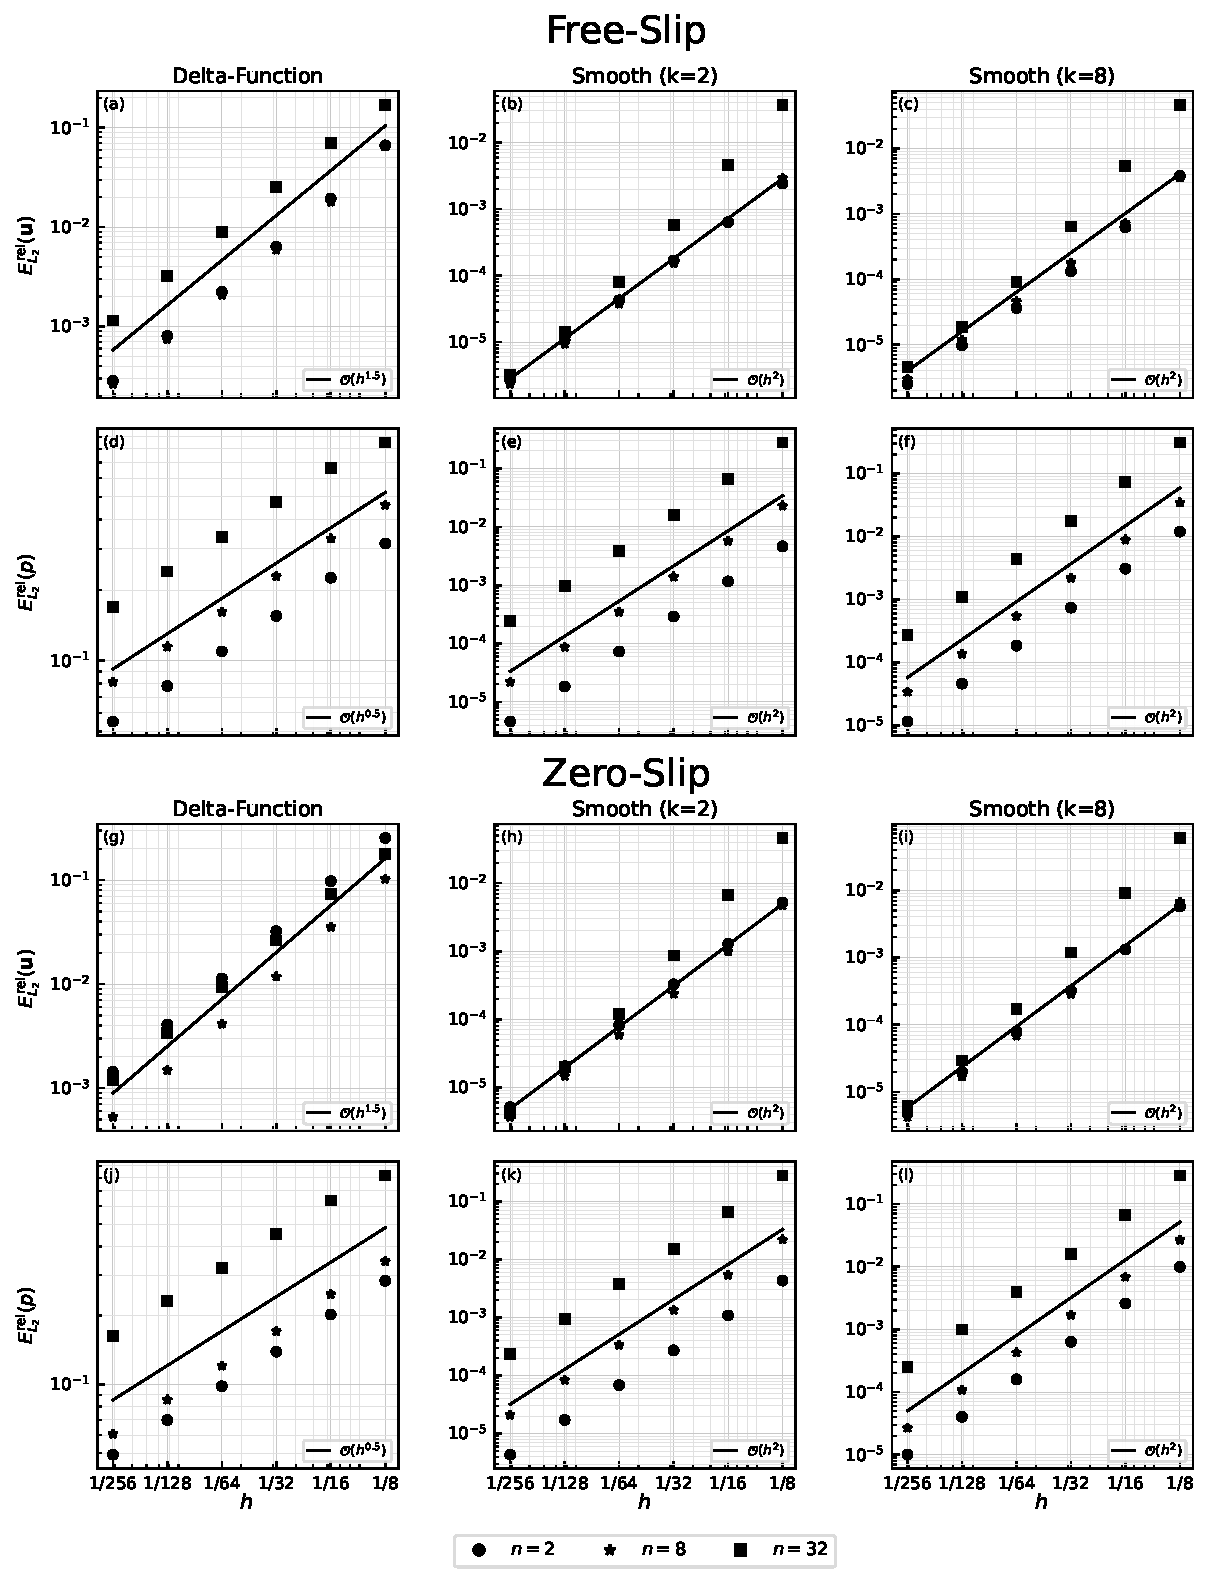
\includegraphics[width=0.95\linewidth,height=0.78\textheight,keepaspectratio]{../annulus/kramer/figure_3_kramer_annulus_convergence.pdf}
\caption{Velocity and pressure convergence for the Kramer annulus benchmark.}
\label{fig:combined_kramer_annulus_convergence}
\end{figure}

\begin{figure}[htb]
\centering

\includegraphics[width=0.95\linewidth,height=0.78\textheight,keepaspectratio]{../spherical/thieulot/figures_4_5_thieulot_convergence.pdf}
\caption{Velocity and pressure convergence for the Thieulot spherical-shell
benchmark.}
\label{fig:combined_thieulot_spherical_convergence}
\end{figure}

\begin{figure}[htb]
\centering
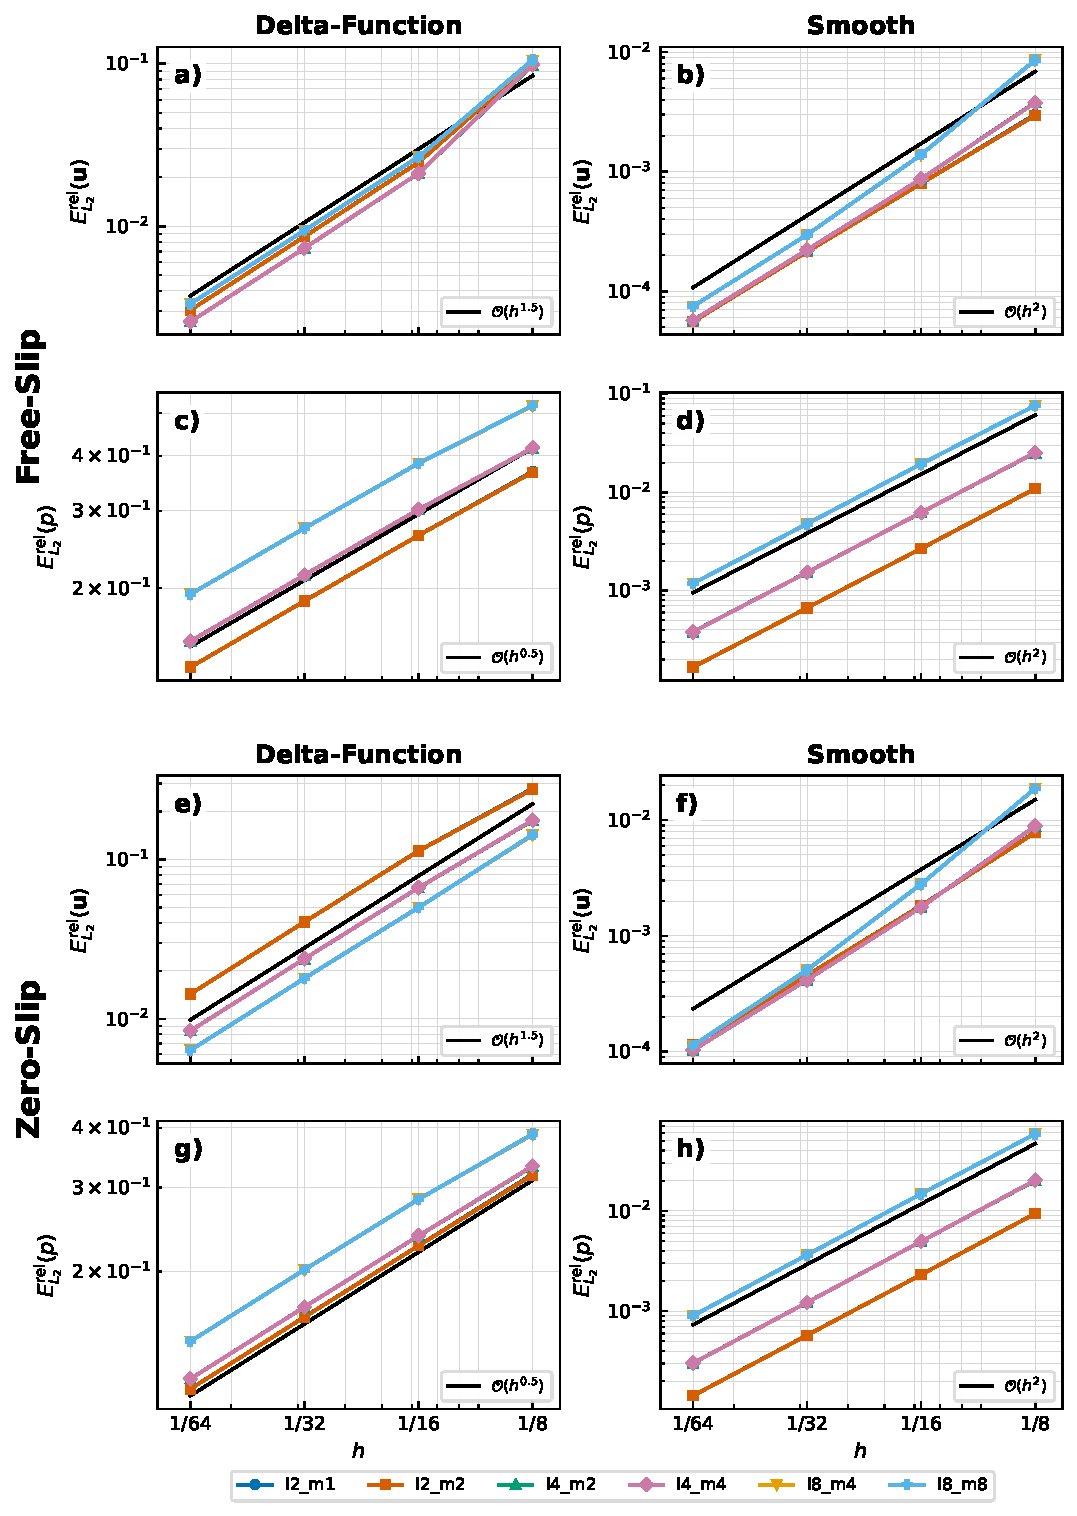
\includegraphics[width=0.95\linewidth,height=0.78\textheight,keepaspectratio]{../spherical/kramer/figure_4_kramer_spherical_convergence.pdf}
\caption{Velocity and pressure convergence for the Kramer spherical-shell
benchmark.}
\label{fig:combined_kramer_spherical_convergence}
\end{figure}

\textbf{results}
For the smooth Thieulot--Puckett annulus benchmark, the Taylor--Hood element
pairs recover the expected hierarchy in the volume \(L_2\) norm. The
\(P_2\times P_1\) pair gives approximately third-order velocity convergence and
second-order pressure convergence. Increasing the polynomial order to
\(P_3\times P_2\) improves the observed rates to approximately fourth order in
velocity and third order in pressure before the finest meshes approach the
error floor. The \(P_2\times P_0\) case gives lower but systematic convergence,
with approximately second-order velocity and first-order pressure behaviour.

For the Kramer annulus benchmark, the observed rates depend primarily on the
regularity of the forcing. Smooth forcing gives second-order pressure
convergence and systematic second-order or better velocity convergence for the
\(P_2\times P_1\) discretisation. When the density forcing is concentrated on an
internal interface, the solution is less regular and the convergence rates
drop to approximately \(O(h^{1.5})\) for velocity and \(O(h^{0.5})\) for
pressure. This reduction is expected from the benchmark construction and is
not interpreted as a failure of the Stokes solve.

The spherical-shell Thieulot benchmark gives the cleanest three-dimensional
smooth-solution result. For the \(P_2\times P_1\) discretisation, both the
constant-viscosity and radially varying viscosity cases approach
\(O(h^3)\) velocity convergence and \(O(h^2)\) pressure convergence in volume
norms. This confirms that the spherical-shell Stokes implementation reproduces
the expected mixed finite-element convergence hierarchy when the analytical
solution is smooth.

The spherical Kramer benchmark shows the same smooth-versus-delta distinction
as the annulus Kramer benchmark. Smooth pressure errors converge close to
\(O(h^2)\), while smooth velocity errors are closer to \(O(h^2)\) than to the
ideal \(P_2\) \(L_2\) rate over the tested mesh sequence. The delta-function
cases recover the expected reduced trends of approximately \(O(h^{1.5})\) in
velocity and \(O(h^{0.5})\) in pressure. Taken together, the annulus and
spherical-shell benchmarks show that the Stokes implementation reproduces the
expected volume-error behaviour for smooth analytical solutions and the
expected reduced convergence when the forcing contains an internal singular
interface.
